\documentclass[11pt]{article}

\usepackage[margin=1in]{geometry}
\usepackage{amsmath,amssymb}
\usepackage{booktabs}
\usepackage{graphicx}
\usepackage{enumitem}
\usepackage{pgfplots}
\usepackage{natbib}
\usepackage{hyperref}
\pgfplotsset{compat=1.17}
\usepgfplotslibrary{groupplots}

\title{Restoring Organs: A Measurement Study of Contact-Based Re-Seating\\
in Long-Horizon Manipulation Chains}
\author{Vihan Aggarwal}
\date{}

\begin{document}
\maketitle

\begin{abstract}
Chaining learned manipulation policies compounds error: a mistake at stage
$k$ shifts every downstream target. We study a recovery primitive, pushing a
part against a physical reference so contact collapses its pose uncertainty
to a fixed state, applied at every stage boundary. The mechanism is the
classical robotic funnel (Mason, 1985; Erdmann and Mason, 1988).
Our question is measurement: does this manufacture the containment
condition funnel composition otherwise needs a mechanics model to certify?
We add a fourth arm, a BATON-style robot-state-only reset, to a bare chain
and a no-contact control. On a 3-D line-up, robot reset alone fails by
$N=4$ (0/10); restore holds $10/10$ at $N=4$, $6/10$ at $N=8$.
Restore contracts per-stage deviation toward a fixed point (ratio 0.206
line-up, 0.387 packing) against near 1.000 for every other arm. Two results
count against us: unifying the primitive to one geometry-derived routine,
needed so one code path serves both tasks, drops the line-up's $N=8$ result
from an earlier task-specific 0.9 to 0.6; and in packing the primitive holds
each stage to 1--8 mm for about eight stages, then fails at $N=12$, a
geometric limit of the push against an already-built structure, not a
policy failure.
\end{abstract}

\section{Introduction}

Chaining a learned manipulation policy across many stages is attractive
because it lets a single skill (pick, place, insert) stand in for a long
task. It is also fragile: if each stage's placement error has some
distribution around the intended target, and stage $k+1$'s target is defined
relative to where stage $k$ actually left the part (as it is in any assembly,
stacking, or kitting task where later parts reference earlier ones), then
error propagates and compounds down the chain. A policy with a comfortable
90\% single-stage success rate is a policy with roughly a 35\% success rate at
ten stages if errors were independent, and considerably worse once
propagation is added, because the effective per-stage target keeps drifting
away from the training distribution.

The manipulation literature has known the fix for forty years: push the part
against something. A sufficiently constraining set of contacts collapses a
whole set of possible poses onto one point, regardless of exactly which pose
the part arrived in, provided it started inside the ``funnel'' that
guarantees convergence to that contact. This is the funnel metaphor of
\citet{mason1985}, formalized as preimage backchaining by
\citet{lozanoperez1984}, extended to purely mechanical (sensorless) part
orientation by \citet{erdmann1988} and \citet{goldberg1993}, generalized to
compositions of funnels by \citet{burridge1999}, and it is also just the
3-2-1 locating principle that every machinist and fixture designer uses, with
its propagation formalized in manufacturing tolerancing as
Stream-of-Variation analysis \citep{jinshi1999,shi2006}. None of this is
new, and we do not claim it is. What we claim, and measure, is narrower:
that this classical, unconditional, detector-free re-seating step, applied
automatically at every stage boundary of a chain whose stage-to-stage policy
is a learned neural network rather than a hand-designed feeder mechanism,
restores long-horizon success where the chain alone and a matched no-op both
collapse to zero.

The reason this needs measuring rather than simply asserting from the
classical theory is that the classical guarantee does not transfer. Funnel
composition guarantees convergence because the designer has a mechanics
model of the part and the fixture and can compute a preimage: the set of
initial configurations that the known dynamics carries into the goal region.
A learned policy has no such model. It has no preimage that can be computed,
so there is no way to certify, in the classical sense, that the part is
inside the basin the physical reference will collapse. Recent long-horizon
manipulation systems that add a recovery or reset step to a learned chain
either do not touch the object at all (BATON, \citet{baton2026}, which
homes the robot's own configuration between VLA subtasks under an LLM
verifier, with no ablation isolating the reset's contribution) or evaluate
recovery within a single stage rather than as a function of chain length
(T-STAR, \citet{lee2021}; SCaR, \citet{scar2024}). We are not aware of prior
work that takes the classical physical re-seating primitive itself,
measures what it does to a learned chain's success as a function of horizon,
and separates the contribution of contact from the contribution of the extra
time and motion the recovery step spends. That is the gap this paper fills.

A note on naming. ``Restoring organ'' is von Neumann's term
\citep{vonneumann1956} for a stage that takes several redundant, possibly
corrupted signal lines and produces one clean line by majority vote. That
is not the mechanism here, and we want to be precise about the difference:
von Neumann's restoring organ removes error through \emph{redundancy}, N
independent copies voting; our restoring step removes error through
\emph{quantization by contact}, a single part is driven against a physical
reference until geometry itself forbids anything but the seated state. The
better analogy is the regenerative repeater in a digital transmission line:
a noisy pulse is not averaged with other pulses, it is snapped to the
nearest valid symbol by a hard nonlinearity (a threshold, here a rigid
contact) and re-transmitted clean. We use ``restoring organ'' for the
push primitive throughout this paper only because that is the name the
codebase and the project use, not as an endorsement of the majority-vote
analogy.

\paragraph{Contributions.}
\begin{enumerate}[leftmargin=*]
  \item We isolate the effect of physical contact from two confounds a
  recovery step also introduces: elapsed time and motion (a motion-matched
  no-op control) and a clean robot starting configuration (a fourth,
  robot-state-only reset arm in the style of BATON). On the 3-D line-up,
  the robot-state reset alone already fails by $N=4$ (0/10 chains); only
  restoring the world state sustains $10/10$ at $N=4$ and $6/10$ at $N=8$.
  The gain is attributable to contact with the part, not to a clean robot
  pose or to elapsed steps.
  \item We give a per-stage mechanism number, not just an endpoint success
  rate: the median ratio of deviation after a stage to deviation at that
  stage's landing. Every non-restoring arm sits at essentially 1.000
  (no contraction) in both robosuite tasks, while restore contracts to
  0.206 (line-up) and 0.387 (packing), and we show this is the right unit
  of measurement because the two tasks fail differently underneath: the
  line-up's bare chain compounds (deviation grows roughly 3 to 156~mm over
  eight stages) while the packing bare chain does not (deviation stays a
  roughly constant 20 to 30~mm because each cube targets its own nominal
  cell), yet restore helps in both regimes.
  \item We give a single geometry-derived reference-finding routine
  (Section~\ref{sec:method}) that reads physical reference faces directly
  from collision geometry rather than from task-specific bookkeeping, and
  show it serves two different task topologies (a 1-D row and a 2-D block)
  unchanged; we also report, honestly, what unifying the primitive costs:
  moving the line-up task from a task-specific fence implementation to this
  shared routine lowers its best-case $N=8$ result from 0.9 to 0.6.
  \item We report a full failure-mode breakdown of what the restore
  primitive does and does not recover (near misses, far misses, and the
  stacked-part failure mode, with a targeted fix), and a set of concrete
  low-level engineering findings (Section~\ref{sec:lessons}) about pushing
  with a parallel gripper that are reusable independent of the main claim.
  \item We report a horizon limit found by extending the packing task to
  $N=12$: restore holds every stage within roughly 1 to 8~mm for about
  eight stages and then fails entirely, because late-stage restores in the
  far row shove the already-finished part of the block by 2 to 35~mm. We
  trace this to a geometric limit of the push primitive against a
  structure it has already built, not to the placement policy, and name
  it explicitly rather than reporting only the success numbers.
  \item We report, honestly, where the primitive breaks: a self-calibration
  routine that estimates contact offsets automatically fails to transfer
  across part size, and the restore's reliability is itself sensitive to
  simulator contact-solver parameters.
\end{enumerate}

\section{Related Work}

\paragraph{Classical funnels and sensorless manipulation.}
\citet{mason1985} introduced the funnel as a metaphor for a control or
mechanical action that maps a region of uncertain initial states to a single
goal state, and \citet{lozanoperez1984} gave the corresponding planning
formalism, preimage backchaining, in which a sequence of commanded motions
is synthesized backward from the goal so that each stage's preimage contains
the previous stage's guaranteed outcome region. \citet{erdmann1988} showed
that purely mechanical actions (tilting a tray) can orient a part with no
sensing at all, and \citet{peshkin1988} formalized fence and edge contacts as
matrix products of configuration maps, giving a compositional algebra for
this kind of uncertainty reduction. \citet{goldberg1993} gave a complete
algorithm for orienting polygonal parts with a sequence of parallel-jaw
squeezes and no sensors, and \citet{burridge1999} generalized funnel
composition to sequential composition of controllers with proven basins of
attraction. In precision manufacturing the same idea appears as the 3-2-1
locating principle, and its propagation through a multi-stage assembly is
modeled by Stream-of-Variation analysis \citep{jinshi1999,shi2006}. All of
this work requires, and provides, a computable model: the preimage, the
configuration map, or the variation transfer function is derived from known
kinematics and contact mechanics. Our contribution is not a new instance of
this theory; it is an empirical account of applying its central primitive,
unconditionally, inside a chain whose per-stage policy is learned and for
which no such model, and hence no such certificate, is available.

\paragraph{Skill chaining and recovery.}
Long-horizon learned manipulation is usually built by chaining short-horizon
skills, and a growing line of work adds explicit recovery behavior between
skills. BATON \citep{baton2026} resets the robot's own configuration
between VLA subtasks, gated by an LLM verifier that decides when a reset is
needed; it reports no ablation isolating what the reset contributes versus
the verifier or the base policy, and it restores the robot, not the world.
Section~\ref{sec:lineup-rerun} supplies that missing ablation for the world-
restoring primitive studied here: a robot-state-only reset arm, run under
the same chain and the same seeds as the other three arms, already fails by
$N=4$ (0/10 chains) on the 3-D line-up, which is the direct empirical
answer to whether a BATON-style robot reset alone could explain the gain we
attribute to restoring the part.
T-STAR \citep{lee2021} trains an adversarial skill-chaining objective so
that individual skills hand off to each other more reliably, which improves
the learned policy itself rather than adding an external physical corrective
step. SCaR \citep{scar2024} addresses skill chaining and recovery within a
learned framework, again evaluated per stage rather than as an explicit
function of chain length. \citet{shao2020} learn to place fixtures that
constrain a part during a downstream operation, which is closely related in
spirit (a designed physical constraint reduces pose uncertainty) but is
solved as a fixture-design problem for a single operation, not as a repeated
primitive re-applied at every stage of an otherwise-learned chain. Amazon's
Stow system \citep{amazonstow2025} uses a corner-sweep motion to
re-canonicalize items during warehouse stowing, which is the same family of
idea (contact quantizes the item's pose against a receptacle corner)
deployed at industrial scale for a single insertion event; we study the
compounding effect of applying the analogous primitive repeatedly across a
chain and quantify how far it extends the chain's horizon.

\paragraph{Long-horizon evaluation.}
\citet{residual2025} benchmark the residual error that accumulates across
long-horizon manipulation chains and argue for measurement protocols that
separate the policy's single-stage competence from its behavior under
compounding error, which is close to the concern of this paper. We adopt a
protocol of up to four arms (bare chain, a motion-matched no-op, a
robot-state-only reset, and restore) specifically so that a change in
success rate can be attributed to contact with the part and not confounded
with the extra wall-clock time and motion, or the clean robot starting
configuration, that any recovery step also introduces; to our knowledge
this decomposition has not been applied to the classical re-seating
primitive before.

\section{Problem Setup and the Arm Protocol}
\label{sec:setup}

Each test bed is a chain of $N$ placement stages. At stage $k$, a policy
(PPO-trained, or a diffusion policy trained by behavior cloning on expert
demonstrations) picks a part and places it at a target pose. In every task
family used here, the target for stage $k$ is defined relative to where the
part from stage $k-1$ \emph{actually} came to rest, not relative to its
nominal pose, so a placement error at stage $k-1$ is inherited by stage $k$
and every stage after it, exactly as in a real assembly or kitting line
where later parts reference earlier ones (a rail, a stop, a neighboring
part) rather than an absolute coordinate frame.

We compare up to four arms, run on identical placements (the same random
seeds and the same underlying policy rollout, so that any two arms differ
only in what happens after the policy has placed the part):

\begin{description}[leftmargin=1.2em]
  \item[bare / no reset] Nothing happens after placement, and (in the
  line-up rerun of Section~\ref{sec:lineup-rerun}) the robot is not homed
  either, so this arm also carries whatever wrist and base drift the chain
  itself accumulates. Errors compound freely.
  \item[robot reset (home)] The end effector is driven back to its exact
  pre-placement position and orientation (the full-pose homing routine of
  Section~\ref{sec:method}) but never touches the part. This is a
  BATON-style reset: it restores the robot's own configuration, not the
  world.
  \item[no-op] A motion-matched control that additionally moves the end
  effector through a trajectory of the same duration and similar spatial
  extent as the restore primitive, on top of the robot reset, but never
  contacts the part. This isolates whether any benefit of restoring is due
  to the physical contact or merely to the extra time and settling the
  restore step spends near the part.
  \item[restore] The restoring organ (Section~\ref{sec:method}): the part
  is pushed against a physical reference (a fixed fence, or whatever part
  is already seated at the previous slot) until contact halts its motion at
  a known pose, followed by the same full-pose robot homing as the other
  arms.
\end{description}

The planar and packing test beds (Sections~\ref{sec:planar},
\ref{sec:packing}) use the three-arm form of this protocol (bare, no-op,
restore); the line-up rerun in Section~\ref{sec:lineup-rerun} uses all four
arms so that the robot-reset and world-restore contributions can be told
apart.

Success is defined per stage (each part within a fixed tolerance of its
nominal cell) and for the whole chain (every stage successful). We report
success rate at fixed horizons $N$ and, for the two robosuite tasks, also
report a censored per-stage reliability bound obtained by raising the
whole-chain success count to the $1/N$ power and applying a one-sided,
95\%, Clopper-Pearson interval \citep{clopperpearson1934} to the resulting
binomial count; the bound is reported as ``at least'' (restore) or ``at
most'' (baselines) because it is only sound in the direction away from the
observed extreme. We use this censored bound rather than a fitted per-stage
success rate $p_{\mathrm{eff}}$ for the baselines because both baselines hit
0 out of 10 chains at $N \geq 4$ in the 3-D task, which leaves $p_{\mathrm{eff}}$
undefined (any $p_{\mathrm{eff}} < 1$ is consistent with zero successes out of
so few trials); the censored bound is defined regardless.

\section{Method}
\label{sec:method}

\subsection{The restore primitive}
The restoring organ closes the gripper into a rigid plate and uses it to
push the part, one axis at a time, against a physical reference until
contact arrests the part's motion, then retreats. Three properties of the
implementation matter for why it works and why it needs to be saturated
control rather than proportional control:

\begin{itemize}
  \item \textbf{Saturated, not proportional, pushing.} A proportional
  controller commands force in proportion to remaining distance to a goal,
  so its commanded force vanishes exactly where a contact-seating push
  needs it most, at the moment of contact. The restore primitive instead
  commands a saturated action toward a target set deliberately past the
  physical reference (an overdrive target), and terminates the push not on
  reaching that overdriven target but on detecting a stall, either the end
  effector's own progress stalling (contact through the plate) or the
  part's own progress stalling (contact through the part), whichever comes
  first, followed by a short unloading phase that relaxes the contact
  before the plate retreats.
  \item \textbf{Geometry-derived references, not task bookkeeping.} Rather
  than hand-coding, for every stage, which object is the fence (the stop
  for the first slot, the previous part for later slots, the rail for the
  first row, the part below for later rows), a single routine
  (\texttt{find\_fences}) scans the scene's collision geometry for the
  nearest static or already-seated box face in $-x$ and in $-y$ from the
  part's nominal pose, subject to a vertical and lateral overlap test, and
  returns those faces as the push targets. This routine is unchanged
  between the 1-D line-up task and the 2-D packing task; the packing task's
  two-axis, two-neighbor reference structure falls out of the same
  geometry query that the line-up task uses for a single stop and a single
  rail, because the query does not know it is being asked about a row
  versus a block.
  \item \textbf{Full-pose homing.} After any restore action the wrist is
  typically 5 to 10 degrees off in yaw and roll from the policy's training
  pose, which the policy cannot observe and which measurably breaks its
  next grasp. We drive the end effector back to the exact position
  \emph{and} orientation it held before the restore (not position only)
  using a quaternion-error controller, identically in every test bed. A
  policy started 30 cm from its home position takes no useful action at
  all, and an 18 degree residual wrist error is enough to break a grasp in
  our tests, which is why full-pose homing, not just position homing, is
  necessary.
\end{itemize}

For parts out of the reachable ``pushable zone'' (tipped, or resting on top
of a neighbor), the primitive first re-grasps the part with jaw orientation
chosen from its measured yaw and drops it back inside the pushable zone
before pushing; see Section~\ref{sec:failure} for when this recovery itself
fails.

\subsection{Self-calibration}
A separate generic implementation (\texttt{rs\_generic.py}) removes the
remaining hand-tuned constants (the offset between the gripper's control
site and the plate's actual contact face) by having the robot creep its
closed fingers onto a part at a known pose until the part moves, once per
axis, and reading off the offset; this is the only quantity in the
primitive that is part-specific, and it is estimated by the robot rather
than measured by hand. All other quantities (push height, approach
clearance, retreat distance) are computed from the part's own extents. The
constants that remain fixed (push amplitude, hold-down bias, stall
thresholds) are properties of the robot and its controller, not of the task
or the part.

\section{Experiments}

\subsection{Planar rig, learned placer (PPO)}
\label{sec:planar}
On a 2-D planar rig with a PPO-trained placement policy, at a fixed chain
length of $N=16$ stages, restore achieves 1.00 success against 0.00 for
both the bare chain and a step-matched no-op control. This holds across a
50$\times$ range of injected placement error at the point of policy output,
which is the strongest single result in this paper precisely because it is
the simplest test bed: two dimensions, one learned policy, and a chain long
enough (16 stages) that the bare chain's cumulative failure probability is
effectively 1 regardless of the exact per-stage error distribution.

\subsection{3-D robosuite line-up rerun on the unified primitive (Panda, diffusion policy)}
\label{sec:lineup-rerun}
The second test bed places 4~cm cubes in a row on a rail with end stops,
using a Panda arm with a parallel gripper and a robomimic diffusion policy
(DDIM, 10 denoising steps) trained by behavior cloning on expert
demonstrations, with a placement tolerance of 8~mm per cube. An earlier
version of this test bed used task-specific fence references and reported
1.0 / 0.9 / 0.9 success at $N = 2,4,8$ (10 seeds); the results below are a
full rerun on the geometry-derived primitive of Section~\ref{sec:method},
the same code that already serves the packing task, so that both tasks in
this paper are now produced by identical restore code. We also add the
robot-state-only reset arm described in Section~\ref{sec:setup}, giving four
arms in total, and apply full-pose homing before every placement except in
the no-reset arm, over 10 paired seeds per cell.

\begin{table}[h]
\centering
\caption{3-D line-up success rate by chain length, unified geometry-derived
primitive, four arms, 10 paired seeds per cell.}
\label{tab:lineup}
\begin{tabular}{lcccc}
\toprule
Arm & $N=2$ & $N=4$ & $N=8$ & steps/stage \\
\midrule
No robot reset          & 0/10  & 0/10  & 0/10 & 255 \\
Robot reset only (home) & 7/10  & 0/10  & 0/10 & 291 \\
Reset + no-contact wander (no-op) & 9/10 & 0/10 & 0/10 & 711 \\
Reset + restore          & 10/10 & 10/10 & 6/10 & 662 \\
\bottomrule
\end{tabular}
\end{table}

Final-row (last-cube) success is restore 1.00 / 1.00 / 0.60 at $N=2,4,8$;
every other arm is 0 at $N=4$ and $N=8$. The censored per-stage bound
(Section~\ref{sec:setup}) is at most 0.509 for no reset, at most 0.713 for
home and for no-op, and at least 0.928 for restore, an ordering consistent
with the observed whole-chain counts. Table~\ref{tab:lineup-contrasts}
reports the pairwise contrasts (exact McNemar on discordant pairs, pooled
over $N$; 95\% bootstrap confidence intervals over pairs).

\begin{table}[h]
\centering
\caption{Pairwise contrasts on the line-up rerun (success rate difference,
discordant pairs, exact McNemar $p$, and mean per-chain deviation change).}
\label{tab:lineup-contrasts}
\begin{tabular}{lcccc}
\toprule
Contrast & $\Delta$ success [95\% CI] & discordant & $p$ & $\Delta$ dev.\ (mm) \\
\midrule
home $-$ no reset    & +0.23 [+0.10, +0.40] & 7:0  & 0.0156   & $-19.6$ \\
no-op $-$ home       & +0.07 [+0.00, +0.17] & 2:0  & 0.5      & $-4.2$ \\
restore $-$ no-op    & +0.57 [+0.37, +0.77] & 17:0 & $1.53\times10^{-5}$ & $-11.9$ \\
restore $-$ home     & +0.63 [+0.47, +0.80] & 19:0 & $3.81\times10^{-6}$ & $-16.2$ \\
\bottomrule
\end{tabular}
\end{table}

Two things follow from this table. First, resetting the robot's own
configuration helps (home beats no reset, $p = 0.0156$) but is far from
sufficient: the robot-reset arm still fails every chain by $N=4$, which is
the direct empirical answer to the BATON-style objection that a clean robot
starting pose might explain the gain we attribute to the part. Second,
spending the same extra time and motion near the part without touching it
(no-op) buys almost nothing over home alone ($p=0.5$, 2 discordant pairs
out of 20); the large, significant gain is specifically restore over no-op
($p = 1.53\times10^{-5}$), i.e., contact, not elapsed time. Section
\ref{sec:horizon} reports the per-stage mechanism behind this table: a
within-stage contraction ratio of 0.206 for restore against 1.000 for every
other arm.

We report the unification cost plainly. The earlier, task-specific-primitive
version of this test bed scored 0.9 at $N=8$; the unified, geometry-derived
primitive used here scores 0.6 at $N=8$, with the drop concentrated in the
final one or two cells of the row. We have not fully isolated why the
shared routine is worse in this one regime; Section~\ref{sec:limitations}
discusses what we do and do not know about the cause.

\subsection{2-D packing horizon sweep ($3\times4$ block, diffusion policy)}
\label{sec:packing}
The third test bed packs cubes into a $3\times4$ block (two contact
references per cell: a left neighbor or stop in $x$, a lower neighbor or
rail in $y$), using a diffusion policy trained separately on 2-D placement
targets over three rows (300 demonstrations, 200 epochs). We compare three
arms (bare, no-op, restore, all with full-pose homing) over 6 paired seeds,
extending the horizon to $N=12$ to test whether the restore arm's success
stays flat past the $N=8$ horizon used in the other two test beds.

\begin{table}[h]
\centering
\caption{2-D packing success rate by chain length, $3\times4$ block, 6
paired seeds per cell.}
\label{tab:pack}
\begin{tabular}{lccccc}
\toprule
Arm & $N=2$ & $N=4$ & $N=8$ & $N=12$ & steps/stage \\
\midrule
None (bare)  & 0/6 & 0/6 & 0/6 & 0/6 & 291 \\
No-op        & 0/6 & 0/6 & 0/6 & 0/6 & 712 \\
Restore      & 6/6 & 6/6 & 4/6 & 0/6 & 679 \\
\bottomrule
\end{tabular}
\end{table}

Final-row success is restore 1.00 / 1.00 / 0.17 / 0.00 at $N=2,4,8,12$;
none and no-op are 0 at every horizon. The censored bound is at most 0.627
for both baselines and at least 0.883 for restore. Restore beats both
baselines decisively (restore $-$ none: $\Delta = +0.67$ [+0.46, +0.83],
16:0 discordant, $p = 3.05\times10^{-5}$, $\Delta$ dev.\ $-14.4$~mm;
restore $-$ no-op: identical success contrast, $\Delta$ dev.\ $-13.9$~mm),
while no-op adds nothing over none ($\Delta = 0.00$, 0:0 discordant, $p=1$,
$\Delta$ dev.\ $-0.5$ [$-2.7$, $+1.1$]~mm): extra motion alone does nothing
in this task either.

Restore's own horizon is limited, and we report the limit and its cause
rather than only the success numbers. Restore holds each stage to roughly 1
to 8~mm of deviation for about eight to nine stages: at $N=8$, 4 of 6
chains keep every individual stage within tolerance, but only 1 of 6 keeps
every cube in tolerance simultaneously at the end, because a later restore
can re-disturb an earlier, already-accepted cube without itself failing its
own stage check. At $N=12$, restore fails all 6 chains, with 28 to 70~mm
single-stage jumps concentrated in the last three to four stages. A
scripted, stage-by-stage trace built while diagnosing this failure shows
the cause: restores in the far row push against the block of cubes already
seated in earlier rows, shifting the finished block by 2 to 35~mm; a
$4\times4$ block showed the same effect (25 to 68~mm in the far column),
and raising the push plate to reduce the disturbance made it worse, not
better. This is a geometric limit of the push primitive against a structure
it has already built, not a failure of the placement policy, and it is the
one honest bound on how far restore extends the horizon in a packing
geometry with zero clearance between finished cells.

\subsection{Horizon and the contraction mechanism}
\label{sec:horizon}
Success rate at fixed $N$ is an endpoint statistic; it does not say what
restore is doing to the error at each stage along the way. We report a
single per-stage number, the within-stage contraction ratio: the median,
over stages, of the deviation measured just after a restore (or after the
no-op or nothing, for the other arms) divided by the deviation at that same
stage's landing (restricted to landings above 2~mm, to avoid dividing by
noise). A ratio near 1.0 means the arm leaves the part where the policy put
it; a ratio well below 1.0 means the arm pulls the part back toward the
reference regardless of where it landed.

\begin{table}[h]
\centering
\caption{Within-stage contraction ratio (median over stages; stage count in
parentheses).}
\label{tab:contraction}
\begin{tabular}{lcc}
\toprule
Arm & line-up & packing \\
\midrule
No reset / none & 1.000 (76) & 0.999 (72) \\
Home            & 1.000 (72) & --- \\
No-op           & 1.000 (75) & 1.001 (72) \\
Restore         & 0.206 (60) & 0.387 (72) \\
\bottomrule
\end{tabular}
\end{table}

Every non-restoring arm sits at essentially 1.000 in both tasks: whatever
the policy or the no-op leaves behind at a stage is what the next stage
inherits. Restore is well below 1.0 in both tasks, but not to the same
degree, and the difference is diagnostic of two different failure regimes
underneath. Figure~\ref{fig:perstage} plots mean per-stage deviation for
every arm in both tasks. In the line-up, the bare chain compounds: mean
deviation grows from 3.1~mm at stage 1 to 155.6~mm at stage 8 ($N=8$), and
home and no-op slow but do not stop this growth (73.4~mm and 56.4~mm at
stage 8), while restore stays within 1.2 to 12.0~mm throughout. In packing,
the bare chain does \emph{not} compound: deviation stays a roughly constant
20 to 30~mm per stage regardless of stage index ($N=12$: 4.1, 17.0, 20.6,
24.6, 12.7, 25.0, 42.8, 18.1, 17.6, 19.9, 29.9, 74.7~mm), because each cube
targets its own nominal cell rather than the previous cube's actual
position, so an error at one stage does not itself relocate the next
stage's target. Restore still helps here (3.3 to 11.0~mm through stage 10),
but its contribution is per-stage correction of a non-growing error, not
arrest of a compounding one, which is why the packing contraction ratio
(0.387) is a weaker number than the line-up's (0.206) even though restore's
absolute deviations are smaller in packing. We read this as strengthening
rather than weakening the paper's claim: the same primitive helps under two
distinct error regimes, unconditional accumulation and unconditional
per-stage noise, for different reasons in each.

We also fit a first-order error recursion, $\epsilon_{k+1} = a\,\epsilon_k +
b$, to the same per-stage deviations. On the line-up ($N=8$): restore
$a = 0.80$ [0.60, 3.13], $b = 1.97$~mm, fixed point 9.8~mm [3.4, 57.9]; home
$a = 1.01$; no-op $a = 0.91$; no reset $a = 0.57$, $b = 46.7$~mm. On packing
($N=12$): restore $a = 0.72$ [0.17, 1.16], $b = 4.33$~mm, fixed point
15.3~mm [7.2, 85.2]; none $a = 0.08$, $b = 25.9$~mm, fixed point 28.1~mm;
no-op $a = -0.02$, $b = 29.4$~mm. The recursion fit is noisy, its confidence
intervals are wide and in one case cross 1, and we report it only because
an attracting fixed point ($a<1$) for restore is the same qualitative story
as the contraction ratio; the contraction ratio in Table~\ref{tab:contraction}
is the number we treat as load-bearing, not the recursion coefficients.

\begin{figure}[h]
\centering
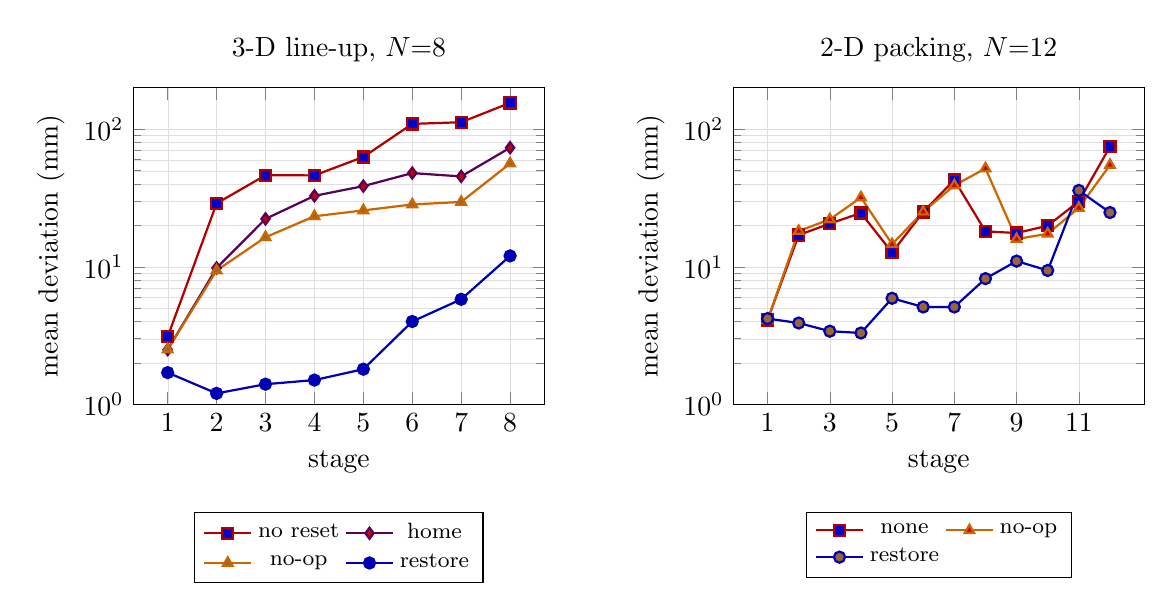
\begin{tikzpicture}
\begin{groupplot}[
  group style={group size=2 by 1, horizontal sep=2.4cm},
  width=6.8cm, height=5.6cm,
  xlabel={stage}, ylabel={mean deviation (mm)},
  ymode=log, ymin=1, ymax=200,
  legend style={font=\footnotesize, at={(0.5,-0.34)}, anchor=north, legend columns=2},
  grid=both, grid style={line width=.1pt, draw=gray!25},
]
\nextgroupplot[title={3-D line-up, $N{=}8$}, xtick={1,2,...,8}]
\addplot+[mark=square*, thick, color=red!70!black] coordinates
  {(1,3.1)(2,28.9)(3,46.3)(4,46.2)(5,62.9)(6,109.4)(7,112.5)(8,155.6)};
\addlegendentry{no reset}
\addplot+[mark=diamond*, thick, color=violet!70!black] coordinates
  {(1,2.5)(2,9.8)(3,22.3)(4,32.8)(5,38.6)(6,48.0)(7,45.4)(8,73.4)};
\addlegendentry{home}
\addplot+[mark=triangle*, thick, color=orange!80!black] coordinates
  {(1,2.5)(2,9.4)(3,16.4)(4,23.3)(5,25.7)(6,28.4)(7,29.6)(8,56.4)};
\addlegendentry{no-op}
\addplot+[mark=*, thick, color=blue!70!black] coordinates
  {(1,1.7)(2,1.2)(3,1.4)(4,1.5)(5,1.8)(6,4.0)(7,5.8)(8,12.0)};
\addlegendentry{restore}
\nextgroupplot[title={2-D packing, $N{=}12$}, xtick={1,3,5,7,9,11}]
\addplot+[mark=square*, thick, color=red!70!black] coordinates
  {(1,4.1)(2,17.0)(3,20.6)(4,24.6)(5,12.7)(6,25.0)(7,42.8)(8,18.1)(9,17.6)(10,19.9)(11,29.9)(12,74.7)};
\addlegendentry{none}
\addplot+[mark=triangle*, thick, color=orange!80!black] coordinates
  {(1,4.1)(2,18.2)(3,22.1)(4,31.9)(5,14.6)(6,25.1)(7,39.0)(8,51.9)(9,15.9)(10,17.4)(11,26.8)(12,54.9)};
\addlegendentry{no-op}
\addplot+[mark=*, thick, color=blue!70!black] coordinates
  {(1,4.2)(2,3.9)(3,3.4)(4,3.3)(5,5.9)(6,5.1)(7,5.1)(8,8.2)(9,11.0)(10,9.4)(11,35.9)(12,24.8)};
\addlegendentry{restore}
\end{groupplot}
\end{tikzpicture}
\caption{Mean per-stage deviation (mm, log scale) versus stage index, all
arms, at the largest horizon run for each task (line-up $N{=}8$, four arms;
packing $N{=}12$, three arms, no separate ``home'' arm). The line-up's bare
chain compounds monotonically; the packing bare chain does not, staying in
a roughly constant 12--75~mm band. Restore stays lowest in both panels
through most of the horizon and only degrades late in the packing panel,
consistent with the far-row block-shove limit described in
Section~\ref{sec:packing}.}
\label{fig:perstage}
\end{figure}

\begin{figure}[h]
\centering
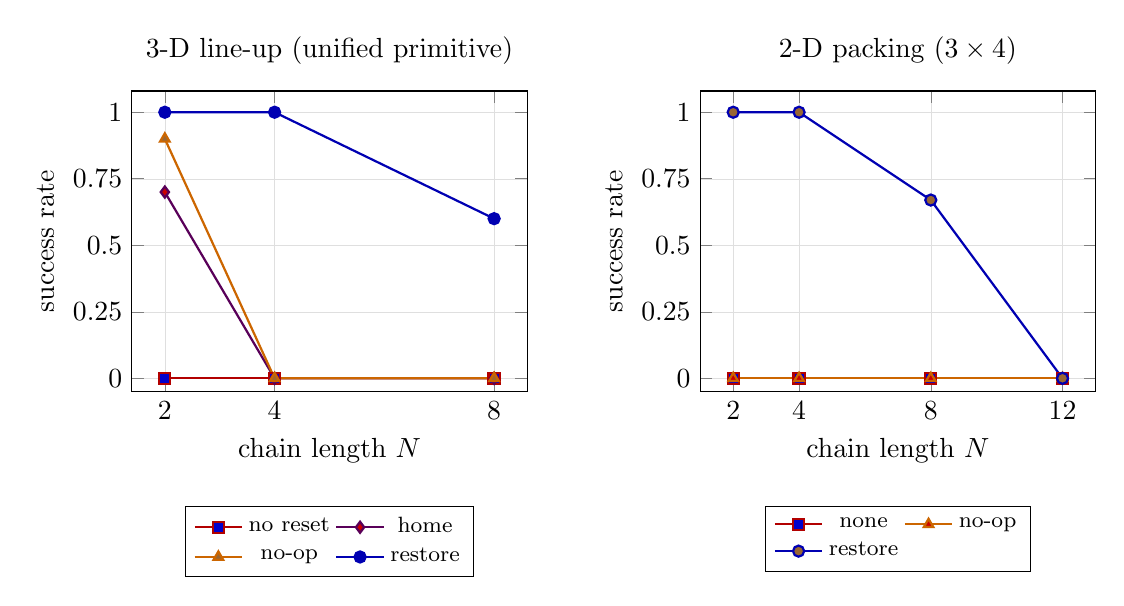
\begin{tikzpicture}
\begin{groupplot}[
  group style={group size=2 by 1, horizontal sep=2.2cm},
  width=6.6cm, height=5.4cm,
  xlabel={chain length $N$}, ylabel={success rate},
  ymin=-0.05, ymax=1.08, ytick={0,0.25,0.5,0.75,1.0},
  legend style={font=\footnotesize, at={(0.5,-0.38)}, anchor=north, legend columns=2},
  grid=both, grid style={line width=.1pt, draw=gray!25},
]
\nextgroupplot[title={3-D line-up (unified primitive)}, xtick={2,4,8}]
\addplot+[mark=square*, thick, color=red!70!black] coordinates {(2,0.0) (4,0.0) (8,0.0)};
\addlegendentry{no reset}
\addplot+[mark=diamond*, thick, color=violet!70!black] coordinates {(2,0.7) (4,0.0) (8,0.0)};
\addlegendentry{home}
\addplot+[mark=triangle*, thick, color=orange!80!black] coordinates {(2,0.9) (4,0.0) (8,0.0)};
\addlegendentry{no-op}
\addplot+[mark=*, thick, color=blue!70!black] coordinates {(2,1.0) (4,1.0) (8,0.6)};
\addlegendentry{restore}
\nextgroupplot[title={2-D packing ($3\times4$)}, xtick={2,4,8,12}]
\addplot+[mark=square*, thick, color=red!70!black] coordinates {(2,0.0) (4,0.0) (8,0.0) (12,0.0)};
\addlegendentry{none}
\addplot+[mark=triangle*, thick, color=orange!80!black] coordinates {(2,0.0) (4,0.0) (8,0.0) (12,0.0)};
\addlegendentry{no-op}
\addplot+[mark=*, thick, color=blue!70!black] coordinates {(2,1.0) (4,1.0) (8,0.67) (12,0.0)};
\addlegendentry{restore}
\end{groupplot}
\end{tikzpicture}
\caption{Success rate versus chain length $N$ for the two robosuite task
families under the unified, geometry-derived restore primitive. The line-up
panel shows all four arms (no reset, home, no-op, restore); the packing
panel has no separate robot-state-only arm, so it shows only three (none,
no-op, restore). The planar (PPO) test bed is not shown on this axis
because it was run at a single horizon ($N=16$, restore 1.00 versus 0.00
for both baselines, held across a 50$\times$ error range) rather than swept
over $N$.}
\label{fig:horizon}
\end{figure}

\section{Failure Analysis}
\label{sec:failure}

An earlier packing run (140 stages per arm, a pilot preceding the results
in Table \ref{tab:pack}) lets us separate what kind of miss the restore
primitive does and does not fix. Restore brought the part back within
tolerance for 69\% of near misses (0.8 to 2~cm off nominal) and for 53\% of
far misses (more than 2~cm off), where the bare chain recovered 0\% of
either class by construction (it takes no corrective action). The
remaining failure class is parts that land stacked on top of a neighbor:
restore recovered only 19\% of these, because the packing grid has zero
clearance between cells and the un-stack routine available at the time
pushed the stacked part sideways in one fixed direction, which has no
guarantee of being the open side once the surrounding cells are partly
filled. Replacing the sideways push with a vertical lift (grasp and raise,
direction-agnostic with respect to which neighboring cells are occupied)
recovered 10 out of 10 stacked cubes in a controlled follow-up test. The
current restore implementation (Section~\ref{sec:method}) uses this lift
for any part detected above the seating plane, which is why it does not
appear in Table \ref{tab:pack}'s results, but the 140-stage breakdown above
predates that fix and is reported here as diagnostic evidence for why the
fix was needed, not as a claim about the final numbers.

A second, distinct failure class, not present at $N \leq 8$ but the sole
cause of failure at $N=12$ (Section~\ref{sec:packing}), is the restore
primitive disturbing its own prior work. A scripted, stage-by-stage trace
built to diagnose the $N=12$ collapse shows that a restore in the far row
pushes against the block of cubes already seated in earlier rows, shifting
that finished block by 2 to 35~mm; a $4\times4$ block reproduced the same
effect (25 to 68~mm of shove in the far column). This is not a miss the
primitive fails to fix; it is the primitive itself re-introducing error
into cells it had already corrected, and it is the reason restore's success
curve turns over at $N=12$ instead of staying flat. Raising the push plate,
the first fix attempted, made the shove worse rather than better, which is
why we report this as an open geometric limitation (Section
\ref{sec:limitations}) rather than a solved failure mode like the stacked-
part case above.

\section{Engineering Lessons}
\label{sec:lessons}

A number of lower-level findings recur across all three test beds and are
useful independent of the paper's central measurement claim.

\begin{itemize}
  \item A proportional (P) controller cannot execute a seating push: its
  commanded force is proportional to remaining error and so vanishes
  exactly at the moment of contact, when force is what is needed. Pushes
  must instead be saturated (constant commanded action) and terminated by
  detecting a contact stall, not by reaching a position target.
  \item The Panda's finger backs are wedge-shaped. A push executed with the
  finger backs lands high on the cube's face, tilts it roughly 17 degrees
  into the fence, and the cube springs back about 7~mm on release. Pushes
  must instead use the flat finger sides, which requires rotating the
  gripper's yaw before each push rather than pushing in whatever orientation
  the arm already holds.
  \item A policy trained from a fixed home pose takes no useful action when
  started 30~cm away from it, and an 18 degree residual wrist orientation
  error is enough to break a grasp, even though the position error at that
  point may be small. Homing after a restore must correct orientation, not
  only position, and must do so identically across every test bed; we
  found no test bed where position-only homing was sufficient.
  \item Measuring a part's pose while the pusher is still in contact with
  it compresses the reading by up to 1~cm, because the part is elastically
  loaded against the fence at the moment of measurement. All pose
  measurements in this paper are taken after the primitive's explicit
  unloading phase, never during a push.
\end{itemize}

\section{Limitations}
\label{sec:limitations}

We report these directly because the framing of this paper is a
measurement claim, and an honest measurement claim includes where the
measurement does not yet reach.

\begin{itemize}
  \item Everything reported here is simulation only (MuJoCo, via robosuite
  and a standalone planar rig); there is no real-robot result in this
  paper. Both robosuite task families use cubes only, and only two task
  topologies (a row, a $3\times4$ block) have been tested.
  \item The push sequence used in the main results (Section~\ref{sec:method})
  is engineered: its constants (approach clearances, push order, retreat
  distances) were set by hand for the specific parts and fixtures used
  here. The self-calibration routine (\texttt{rs\_generic.py}) removes the
  hand-measured contact offset, but does not transfer to unseen part sizes
  without retuning the constants that remain fixed: a scripted transfer
  test scored 2 out of 3 on the tuned 2~cm cube, 1 out of 3 on a 1.5~cm
  cube, 0 out of 3 on a 3~cm cube, and 0 out of 3 on an oblong
  $3\times2\times2$~cm block. The most likely cause is that push amplitude
  and stall thresholds, both currently fixed robot-controller constants,
  do not scale with the part's mass, so they under- or over-drive parts far
  from the size they were tuned on.
  \item Restore success is itself sensitive to the physics solver's contact
  parameters. In a scripted probe across MuJoCo contact time constants of
  0.02, 0.010, and 0.005~s and friction multipliers of 0.5 and 2.0, restore
  success went 4/4, 0/4, 1/4, 4/4, 0/4 across the five parameter settings
  tested, an unstable pattern that is not currently explained and that
  means the reported success rates should be read as holding for the
  solver configuration used in this paper, not as solver-independent.
  \item Unifying the restore primitive cost the line-up task some
  performance. Tables \ref{tab:lineup} and \ref{tab:pack} are now produced
  by identical restore code, but the unified, geometry-derived routine
  scores 0.6 at $N=8$ on the line-up where the earlier, task-specific-fence
  version of the same test bed scored 0.9. We have not fully isolated the
  cause; the geometry query returns a coarser or differently placed fence
  face than the hand-coded reference did in a minority of cells, and this
  is the most direct candidate, but we have not run the scripted comparison
  needed to confirm it. Readers should treat 0.9 as an upper bound achieved
  by a less general implementation, not as a number the unified primitive
  is known to be capable of.
  \item Restore's horizon is bounded by a geometric limit of the push
  primitive itself, not by the placement policy. In the packing task, a
  restore in a later row can shove cubes already seated in an earlier row
  (Section~\ref{sec:failure}), and this is the sole cause of the collapse
  to 0/6 at $N=12$: individual stages still land within a few millimeters
  through most of the chain, but the finished part of the structure does
  not stay still while later stages are completed. This limitation is
  specific to packing geometries with zero clearance between finished
  cells; the line-up task, where each new cube is placed beyond the
  existing row rather than into it, does not exhibit it at the horizons
  tested here ($N \leq 8$).
\end{itemize}

\section{Conclusion}

Pushing a part against a physical reference is not a new idea; it is the
oldest idea in robotic manipulation for handling pose uncertainty, and its
classical form comes with a certificate (a computable preimage) that a
learned policy cannot provide. What we measure here is that applying the
primitive anyway, unconditionally and at every stage boundary, restores
long-horizon success in three independent learned test beds, and that the
gain is specifically attributable to contact with the part rather than to
a clean robot starting pose or to the extra time and motion a recovery step
also spends: a robot-state-only reset in the style of BATON already fails
by $N=4$ on the 3-D line-up, and a motion-matched no-op buys almost nothing
over that reset. The clearest single number behind this claim is not an
endpoint success rate but a per-stage one, the within-stage contraction
ratio: restore pulls deviation back toward a fixed point (0.206 in the
line-up, 0.387 in packing) where every other arm leaves it unchanged
(essentially 1.000). The primitive is not free of its own fragility, and we
have tried to report where it breaks rather than around it. Unifying it to
a single geometry-derived reference routine, needed so one code path serves
both tasks, costs the line-up task real performance (0.9 down to 0.6 at
$N=8$), and the packing task's horizon is bounded by a geometric limit we
did not anticipate: a restore in a later row shoving cubes already seated
in an earlier one, which collapses success entirely by $N=12$ even though
individual stages keep landing within a few millimeters. Neither of these
is fixed in this paper; both are named, measured, and left as concrete
next steps rather than smoothed over.

\section{Future Work}
\label{sec:todo}

Two further gaps remain unresolved by the experiments in this paper.

\begin{enumerate}[leftmargin=*]
  \item \textbf{Pushes that do not load the finished structure.} The
  packing horizon limit (Sections~\ref{sec:packing}, \ref{sec:failure}) is
  caused by the push primitive shoving already-seated parts, not by the
  placement policy; a push order or contact strategy that never applies
  force through a finished sub-assembly (for example, always pushing away
  from, rather than through, previously completed rows) is the direct fix
  and is untested here.
  \item \textbf{Mass-scaled push parameters.} The self-calibration
  routine's failure to transfer across part size (Section
  \ref{sec:limitations}) is most likely explained by push amplitude and
  stall thresholds that do not scale with the part's mass; scaling these
  constants from the part's measured or nominal mass, rather than holding
  them fixed, is the natural next experiment and has not been run.
  \item \textbf{An external long-horizon benchmark.} We scoped a port to
  CALVIN and to FurnitureBench. CALVIN is the more feasible target because
  it exposes ground-truth object and joint poses directly and has public
  pretrained checkpoints to chain, at an estimated three to four weeks of
  effort, but its failures may turn out to be mostly semantic or grasp
  failures rather than the geometric drift this primitive addresses, so a
  short scripted check of that question should precede any full port;
  FurnitureBench is a better mechanical fit (parts are pushed into a fixed
  corner fence) but costs five to eight weeks and a dedicated Linux GPU
  machine because of its deprecated simulator.
  \item \textbf{A real-robot confirmation.} Every result in this paper is
  simulation only. Confirming the contraction effect on hardware, even at
  a single horizon on one task, is the outstanding step before any of
  these numbers can be read as more than a simulation finding.
\end{enumerate}

\begin{thebibliography}{99}

\bibitem[Amazon Robotics, 2025]{amazonstow2025}
Amazon Robotics.
\newblock Learned corner-sweep re-canonicalization for robotic stowing.
\newblock \emph{arXiv:2505.04572}, 2025.

\bibitem[BATON, 2026]{baton2026}
Anonymous.
\newblock BATON: restoring robot configuration between VLA subtasks with an
LLM verifier.
\newblock \emph{arXiv:2608.16889}, 2026.

\bibitem[Burridge et al., 1999]{burridge1999}
R.~R. Burridge, A.~A. Rizzi, and D.~E. Koditschek.
\newblock Sequential composition of dynamically dexterous robot behaviors.
\newblock \emph{International Journal of Robotics Research}, 18(6):534--555,
1999.

\bibitem[Clopper and Pearson, 1934]{clopperpearson1934}
C.~J. Clopper and E.~S. Pearson.
\newblock The use of confidence or fiducial limits illustrated in the case
of the binomial.
\newblock \emph{Biometrika}, 26(4):404--413, 1934.

\bibitem[Erdmann and Mason, 1988]{erdmann1988}
M.~A. Erdmann and M.~T. Mason.
\newblock An exploration of sensorless manipulation.
\newblock \emph{IEEE Journal of Robotics and Automation}, 4(4):369--379,
1988.

\bibitem[Goldberg, 1993]{goldberg1993}
K.~Y. Goldberg.
\newblock Orienting polygonal parts without sensors.
\newblock \emph{Algorithmica}, 10(2--4):201--225, 1993.

\bibitem[Jin and Shi, 1999]{jinshi1999}
J.~Jin and J.~Shi.
\newblock State space modeling of sheet metal assembly for dimensional
control.
\newblock \emph{ASME Journal of Manufacturing Science and Engineering},
121(4):756--762, 1999.

\bibitem[Lee et al., 2021]{lee2021}
Y.~Lee, E.~S. Hu, and J.~J. Lim.
\newblock Adversarial skill chaining for long-horizon robot manipulation via
terminal state regularization.
\newblock In \emph{Conference on Robot Learning (CoRL)}, 2021.

\bibitem[Lozano-P\'{e}rez et al., 1984]{lozanoperez1984}
T.~Lozano-P\'{e}rez, M.~T. Mason, and R.~H. Taylor.
\newblock Automatic synthesis of fine-motion strategies for robots.
\newblock \emph{International Journal of Robotics Research}, 3(1):3--24,
1984.

\bibitem[Mason, 1985]{mason1985}
M.~T. Mason.
\newblock The mechanics of manipulation.
\newblock In \emph{IEEE International Conference on Robotics and Automation
(ICRA)}, pages 544--548, 1985.

\bibitem[Peshkin and Sanderson, 1988]{peshkin1988}
M.~A. Peshkin and A.~C. Sanderson.
\newblock Planning robotic manipulation strategies for workpieces that slide.
\newblock \emph{IEEE Journal of Robotics and Automation}, 4(5):524--531,
1988.

\bibitem[Residual Benchmark, 2607]{residual2025}
Anonymous.
\newblock Benchmarking the residual: measuring compounding error in
long-horizon manipulation chains.
\newblock \emph{arXiv:2607.27283}, 2025.

\bibitem[SCaR, 2024]{scar2024}
Anonymous.
\newblock SCaR: skill chaining and recovery for long-horizon manipulation.
\newblock In \emph{Advances in Neural Information Processing Systems
(NeurIPS)}, 2024.

\bibitem[Shao et al., 2020]{shao2020}
L.~Shao, T.~Migimatsu, and J.~Bohg.
\newblock Learning to scaffold the development of robotic manipulation
skills.
\newblock In \emph{IEEE International Conference on Robotics and Automation
(ICRA)}, 2020.

\bibitem[Shi, 2006]{shi2006}
J.~Shi.
\newblock \emph{Stream of Variation Modeling and Analysis for Multistage
Manufacturing Processes}.
\newblock CRC Press, 2006.

\bibitem[von Neumann, 1956]{vonneumann1956}
J.~von Neumann.
\newblock Probabilistic logics and the synthesis of reliable organisms from
unreliable components.
\newblock In C.~E. Shannon and J.~McCarthy, editors, \emph{Automata
Studies}, pages 43--98. Princeton University Press, 1956.

\end{thebibliography}

\end{document}
